\documentclass[a4paper, 12pt]{article}
\usepackage[utf8]{inputenc}
\usepackage[english,russian]{babel}
\usepackage[warn]{mathtext}
\usepackage{graphicx}
\usepackage{float}
\usepackage{multirow}
\restylefloat{table}
\usepackage{amsmath}
\usepackage{floatflt}
\usepackage[T2A]{fontenc}
\usepackage[left=20mm, top=20mm, right=20mm, bottom=20mm, footskip=10mm]{geometry}

\tolerance 1414
\hbadness 1414
\emergencystretch 1.5em
\hfuzz 0.3pt        % размер максимального переполнения без warning'a
\widowpenalty=10000 % запрещает одиночную строку абзаца в начале страницы
\vfuzz \hfuzz
\raggedbottom       % если на странице мало содержимого, добавить пустое место в конце, а не в середине страницы



\begin{document}

\begin{titlepage}
	\centering
	\vspace{5cm}
	{\scshape\LARGE московский физико-технический институт (национальный исследовательский университет) \par}
	\vspace{6cm}
	{\scshape\Large Лабораторная работа 4.7.2 \par}
	{\huge\bfseries Эффект Поккельса \par}
	\vspace{1cm}
	\vfill
\begin{flushright}
	{\large Б03-102}\par
	\vspace{0.3cm}
	{\LARGE Куланов Александр}
\end{flushright}
	

	\vfill


	Долгопрудный, 2023 г.
\end{titlepage}

\begin{itemize}
	\item \textbf{Цель работы:} исследовать интерференцию рассеянного света, прошедшего кристалл; наблюдать изменение характера поляризации света при наложении на кристалл электрического поля.
    \item \textbf{В работе используются:} гелий-неоновый лазер, поляризатор, кристалл ниобата лития, матовая пластина, экран, источник высоковольтного переменного и постоянного напряжения, фотодиод, осцилограф, линейка.
\end{itemize}
\section{Теоретические сведения}

Эффектом Поккельса называется изменение показателя преломления света в кристалле под действием электрического поля, причём это изменение пропорционально напряжённости электрического поля. Как следствие эффекта Поккельса в кристалле появляется двойное лучепреломление или меняется его величина, если кристалл был двулучепреломляющим в отсутствие поля.

Изменение показателя преломления кристаллов под действием внешнего электрического поля происходит исключительно за счёт анизотропных свойств кристаллов. Под действием постоянного электрического поля электроны смещаются в сторону того или иного иопа (в случае кристалла ниобата лития $\mathrm{LiNbO}_3-$ это ион $\mathrm{Li}$ или $\mathrm{Nb}$ ), при этом меняется поляризуемость среды и связаппый с ней показатель преломления. В первом приближении это изменение линейно относительно внешпего электрического поля. Эффект Поккельса может набльдаться только в кристаллах, не обладающих центром симметрии. Вследствие линейности эффекта относительно внешнего поля $E_{эл}$ при изменении паправления поля на противоположное должеп меняться на противоположный и знак изменения показателя преломления $\Delta n$. Но в кристаллах с цептром симметрии это невозможно, так как оба взаимно противоположных паправления внешшего поля физически эквивалептиы. Кристалл можно поместить между двумя скрещенными поляроидами таким образом, что в отсутствие внешнего электрического поля пропускание света системой будет равно нуло. При подаче па кристалл внештего поля появится паведёшне двулучепреломлепие, которое измепит поляризациюо прошедшего через кристалл света, и такая система начнёт пропускать свет. На этом прищципе осповапы мпогочисленшые примепения эффекта Поккельса в
лазерной технике для оптических модуляторов, затворов и других устройств, управляющих лазершым излучением. Поскольку эффект Поккельса связан с изменением электронной поляризуемости под действием электрического поля, то он практически безынерционен - быстродействие устройств на его основе меньme $10^{-9} \mathrm{c}$.

Рассмотрим сначала кристалл в отсутствие внешнего электрического полs. Кристали ниобата лития является одноосным кристаллом, то есть кристаллом, оптические свойства которого обладают симметрией вращения относительно некоторого одного направления, называемого оптической осъю $Z$ кристалла. Для световой волы, вектор электрического поля $\vec{E}$ которой перпендикулярен оси $Z$, показатель преломления равен $n_o$, а для волны, вектор $\vec{E}$ которой располатается вдоль оси $Z$, он равен $n_e$, причём $n_e<n_o$, т. е. $\mathrm{LiNbO}_3-$ «отрицательный кристалля. В общем случае, когда луч света распространяется под углом $\theta$ к оптической оси $Z$ (рис. 1), существуют два собственных значения показателя преломления $n_1$ и $n_2$ : если световой вектор $\vec{E}$ перпендикулярен плоскости $(\vec{k}, \vec{Z})$, где $\vec{k}-$ волновой вектор луча, то волна называется обыкновенной («о» - ординарная), а показатель преломления $n_1$ равен $n_o$ и не зависит от угла $\theta$; когда световой вектор $\vec{E}$ лежит в плоскости $\vec{k}, \vec{Z}$ - это необыкновенная (ке» - экетраординарная) волна, при этом показатель преломления $n_2$ зависит от угла $\theta$ и определяется уравнением
\begin{equation}
\frac{1}{n_2^2}=\frac{\cos ^2 \theta}{n_o^2}+\frac{\sin ^2 \theta}{n_e^2} .
\end{equation}
Нетрудно видеть, что при $\theta=0$ и $90^{\circ}$ n $n_2$ равен $n_o$ и $n_{\text {с  }}$ соответственно.

Если перед кристаллом, помещёным между скрещениыми поляроидами (рис. 1), расположить линзу или матовуюо пластинку, после которых лучи будут рассеиваться под различными углами, то на экране, расположенном за поляроидом, мы увидим тёмшые концентрические окружности (коноскопическую картину) результат интерференции обыкиовенной и необыкновеший волн, точнее, проекцио их электрических полей на разрешёние паправлепие выходпого поляроида. В пашем эксперимепте используется лазер, излучение которого поляризовано, поэтому входиой по.ляоид можно пе ставнть.

Разность фаз между обыкновенной и необыкновепнй волнами, приобретаемая при прохождепии через кристалл длиной l. равна
\begin{equation*}
\Delta \varphi=\frac{2 \pi}{\lambda} \cdot l \cdot\left(n_1-n_2\right)
\end{equation*}
Для обыкноветного луча $n_1=n_0$ и не зависит от угла $\theta$ между направлением луча и осью Z. Для необыкновениого луча $n_2$ зависит от угла $\theta$ и определяется уравнепием (1). Считая, что $n_c$ и $n_0$ отличаются иезначительно, для мальх углов $\left(\sin \theta \approx \theta, \cos \theta \approx 1-\theta^2 / 2\right)$ получаем $n_2=n_o-\left(n_o-n_c\right) \theta^2$. Таким образом,
\begin{equation*}
\delta=\frac{2 \pi}{\lambda} l\left(n_0-n_c\right) \theta^2
\end{equation*}

\begin{figure}[H]
    \centering
    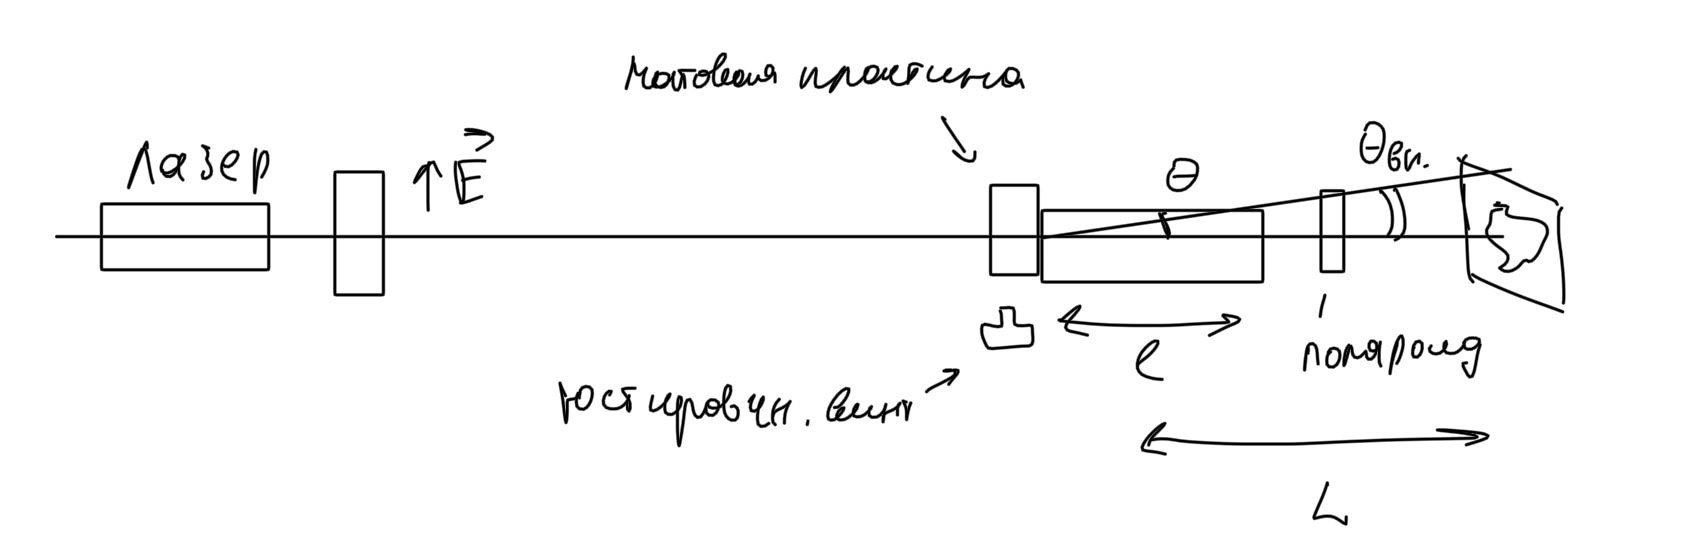
\includegraphics[width=1\textwidth]{ris1}
    \caption{Наблюдение интерференционной картины}
    \label{fig:ris1}
\end{figure}

Направлениями постоянной разности фаз служат конусы $\theta=$ = const, поэтому интерференционная картина представляет собой концентрические окружности. Интерференционые кольца перерезаны тёмным «мальтийским крестом», который выделяет области, где интерферениия отсутствует. В этих направлениях распространяется только одна поляризованная волна (обыкновенная или необыкновенная). При повороте выходного поляроида (анализатора) па $90^{\circ}$ картина меняется с позитива на негатив: везде, где были светлые места, появляюотся тёмпые и наоборот.

Для случая, когда разрешённое направление анализатора перпепдикулярно поляризации лазерного излучения (скрепепные поляризации). найдём радиус тёмпого кольца с помером $m$. . Дл луча. илушего вдоль оси $Z(m=0)$, показатеми преломления для двух воли совпадают, сдвит фаз межлу пими равен пуло, поляризация излучения па выходе остаётся такой же. как на входе, и луч пе проходит через анализатор. Картина пе изменится при сдвиге фаз между обыкновепой и пеобыкновенпой вомной, кратном $2 \pi$. Поэтому для $m$-го тёмиого кольща $\delta=2 \pi m и \pi и \delta$ $=\frac{2 \pi}{\lambda} l\left(n_o-n_e\right) \theta^2=2 \pi m$. Если $L$ расстоsние от цеттра кристалла до экрана, то, учитывая закон преломления (закон Снелииуса) па границе кристалла, при малых углах $\theta_{\text {висши }}=n_0 \theta$ (pис. 1) получаем выражепие для радиуса кольца:
\begin{equation}
r_m^2=\frac{\lambda}{l} \frac{\left(n_o L\right)^2}{\left(n_0-n_e\right)} m
\end{equation}
Измеряя радиусы колец, можпо найти разность $\left(n_o-n_c\right)$ двулучепреломление кристалла.

Представим теперь, что мы поместили кристалл в постоянное электрическое поле $E_{э л}$, направленное вдоль оси $X$, перпендикулярной оптической оси кристалла $Z$. Луч света распространяется вдоль оси $Z$, при этом для любой поляризации в отсутствие внешнего поля показатель преломления равен $n_o$. Свойства симметрии кристалла и его электрооптический тензор таковы, что в результате линейного электрооптического эффекта (эффекта Поккельса) в плоскости $(X, Y)$ возникают два главных направлепия \& и $\eta$ под углами $45^{\circ}$ к осям $X$ и $Y$ (рис. 2) с показателями преломления $\left(n_0-\Delta n\right)$ и $\left(n_0+\Delta n\right)$, то есть появляются «медленная» и «быстрая» ось, причём $\Delta n=A \cdot E_{\text {эл }}(A-$ некая константа, зависящая только от типа кристалла).

Пусть свет на входе в кристалл поляризован вертикально, а на выходе стоит анализатор, пропускающий горизонтальную поляризацик. Разложим исходиый световой вектор $E=E_0 e^{i(\omega t-k z)}$ по осям \& и $\eta: E_{\xi}=E_\eta=E_0 / \sqrt{2}$. После прохождения кристалла между векторами $E_{\varepsilon}$ и $E_\eta$ появится разность фаз
\begin{equation*}
\delta=\frac{2 \pi l}{\lambda} 2 \Delta n=\frac{4 \pi l}{\lambda} A E_{9 \pi}=\frac{4 \pi}{\lambda} \frac{l}{d} A U,
\end{equation*}
где $U=E_{3 \wedge} \cdot d-$ напряжение па кристалле, $d-$ размер кристалла в поперечном направлении. Результирующее поле после анализатора это сумма проекций $E_{\xi}$ и $E_\eta$ на направление $X$, т. е.
\begin{equation*}
E_{\mathrm{Bux}}=\frac{E_0}{2} e^{i(\omega t-k l)}\left(e^{i \delta / 2}-e^{-i \delta / 2}\right)=E_0 e^{i(\omega t-k l)} \sin \left(\frac{\delta}{2}\right) \text {. }
\end{equation*}
Интенсивность света пропорциональна квадрату модуля вектора электрического поля в волне:
\begin{equation*}
I_{\text {max }} \sim E E^*=E_0^2 \sin ^2\left(\frac{\delta}{2}\right) \text {, }
\end{equation*}
поэтому
\begin{equation}
I_{\mathrm{max}}=I_0 \sin ^2\left(\frac{\delta}{2}\right)=I_0 \sin ^2\left(\frac{\pi}{2} \frac{U}{U_{X / 2}}\right) \text {. }
\end{equation}
Здесь
\begin{equation}
U_{\lambda / 2}=\frac{\lambda}{4 A} \frac{d}{l}
\end{equation}
- так называемое полуволнове напряжсение н имеет тот смысл, что при $U=U_{\lambda / 2}$ сдвиг фаз между двумя волнами, соответствуюошими двум собственным поляризациям. $\delta=\pi$ (разность хода равна $\lambda / 2$ ), и интенсивность света па выходе анализатора достигает максимума. Это следует из (3).

\begin{figure}[H]
    \centering
    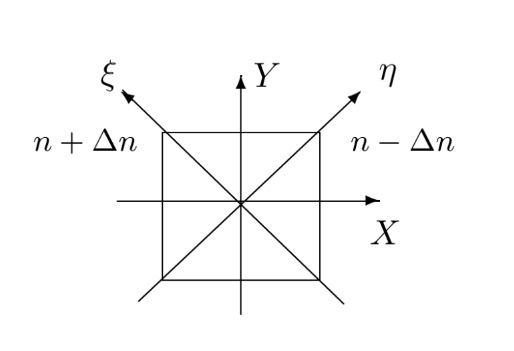
\includegraphics[width=0.5\textwidth]{ris2}
    \caption{Эффект Поккельса}
    \label{fig:ris2}
\end{figure}

Студенту предлагается показать, что при параллелыных полsризащиях лазера и анализатора
\begin{equation}
I_{\mathrm{max}}=I_0 \cos ^2\left(\frac{\pi}{2} \frac{U}{U_{\lambda / 2}}\right)
\end{equation}

\begin{figure}[H]
    \centering
    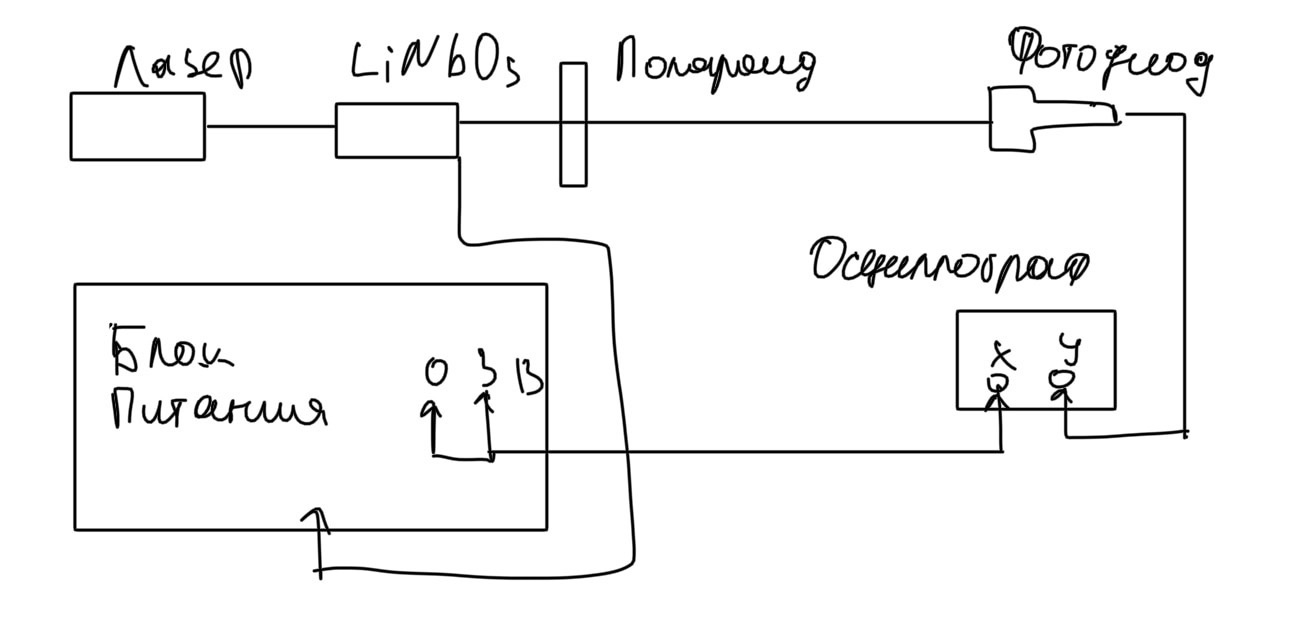
\includegraphics[width=1\textwidth]{ris3}
    \caption{Схема установки}
    \label{fig:ris3}
\end{figure}

\section{Экспериментальная установка}
Оптическая часть установки представлена на рис. 1. Свет гелий-неонового лазера, поляризоватный в вертикальной плоскости, проходя сквозь матовую пластинку, рассеивается и падает на двоякопреломляюший кристалл под различными углами. Кристалл ниобата лития с размерами $3 \times 3 \times 26$ мм вырезан вдоль оптической оси $Z$. На экране, расположенном за скрещенньм поляроидом, видна интерференщионияя картина.

Для $\lambda=0,63$ мкм (длина волны гелий-неонового лазера) в ниобате лития $n_o=2,29$.

Убрав рассеиваюощую пластинку и подавая на кристалл постоянное напряжение, можно величиной папряжепия влиять на поляризацию луча, вышедшего из кристалла.
-Заменив экран фотодиодом (рис. 3) и подав на кристалл переменное напряжение, можно исследовать поляризацию луча с помощыь осциллографа.
\section{Выполнение работы}
\subsection*{Определение разности показателей преломления}
Получим на экране интерференционную картину при $L = 80 \pm 1 см$. Измерим радиусы темных колец с помощью линейки. По полученным данным построим график $f(m)$.

\begin{table}[H]
	\centering
	\begin{tabular}{|c|c|c|c|c|c|c|c|c|}
	\hline
	m         & 1 & 2     & 3  & 4     & 5     & 6     & 7     & 8     \\ \hline
	r, см     & 3 & 4,2   & 5  & 5,8   & 6,5   & 7,3   & 7,8   & 8,3   \\ \hline
	$r^2$, см & 9 & 17,64 & 25 & 33,64 & 42,25 & 53,29 & 60,84 & 68,89 \\ \hline
	\end{tabular}
	\caption{Данные для интерференционной картины}
	\label{tab:data1}
\end{table}
\begin{figure}[H]
    \centering
    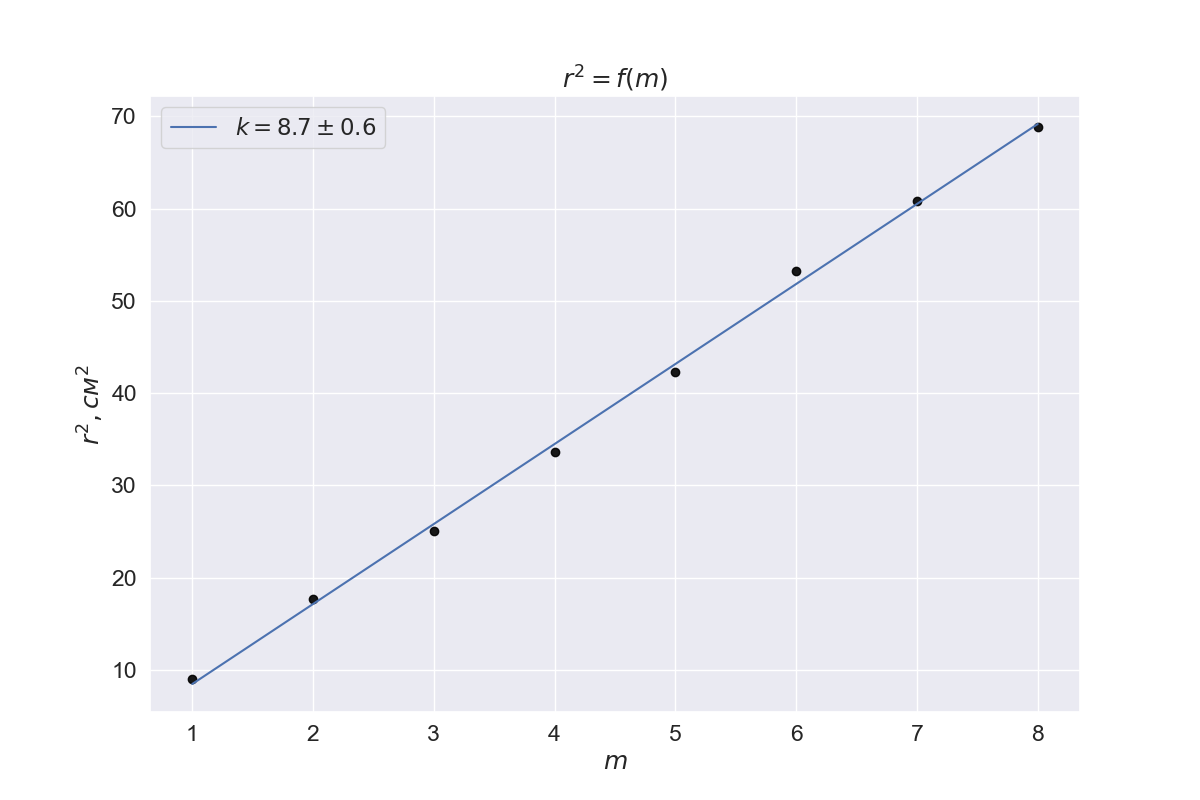
\includegraphics[width=1\textwidth]{plot1.png}
    \caption{Зависимость квадрата радиуса от номера радиуса}
    \label{fig:plot1}
\end{figure}
Получаем, что наклон лучшей прямой составляет $8.7 \pm 0.6$ кв. см. Из формулы (2), получаем:
\begin{equation}
	r_m^2=\frac{\lambda}{l} \frac{\left(n_o L\right)^2}{\left(n_0-n_e\right)} m = km
\end{equation}
У нас $n_0 = 2.29$, $\lambda = 0.63$ мкм, $l = 26$ мм
\begin{equation}
	n_0 - n_e = \frac{\lambda (n_0 L)^2}{lk} = 0.09 \pm 0.01
\end{equation}
\subsection*{Определение полуволнового напряжения}
Поставим поляроид в перпендикулярное положение. Получим значения напряжения, для которого интенсивность максимальна. Это будет напряжение $U_{\lambda/2} = 510 \pm 15$ В. Аналогично, для минимальной интенсивности получим напряжение $U_{\lambda} = 930 \pm 15$ В.
Если повернуть поляроид на 90 градусов, то картина изменится на противоположную: при полуволновом напряжении будет минимум, при целоволновом максимум и т.д.

Если же подать на кристалл напряжение, равное половине $U_{\lambda/2}$, то поляризация станет круговой. Опыт показал, что это действительно так.

Далее, с помощью осциллографа так же померяем полуволновое напряжение.
\begin{equation*}
	U_{\lambda/2} = (58 дел - 30 дел) * 15 В = 420 \pm 15 \text{ В}
\end{equation*}
Картины фигур Лиссажу на экарне осциллографа:

\begin{figure}[H]
    \centering
    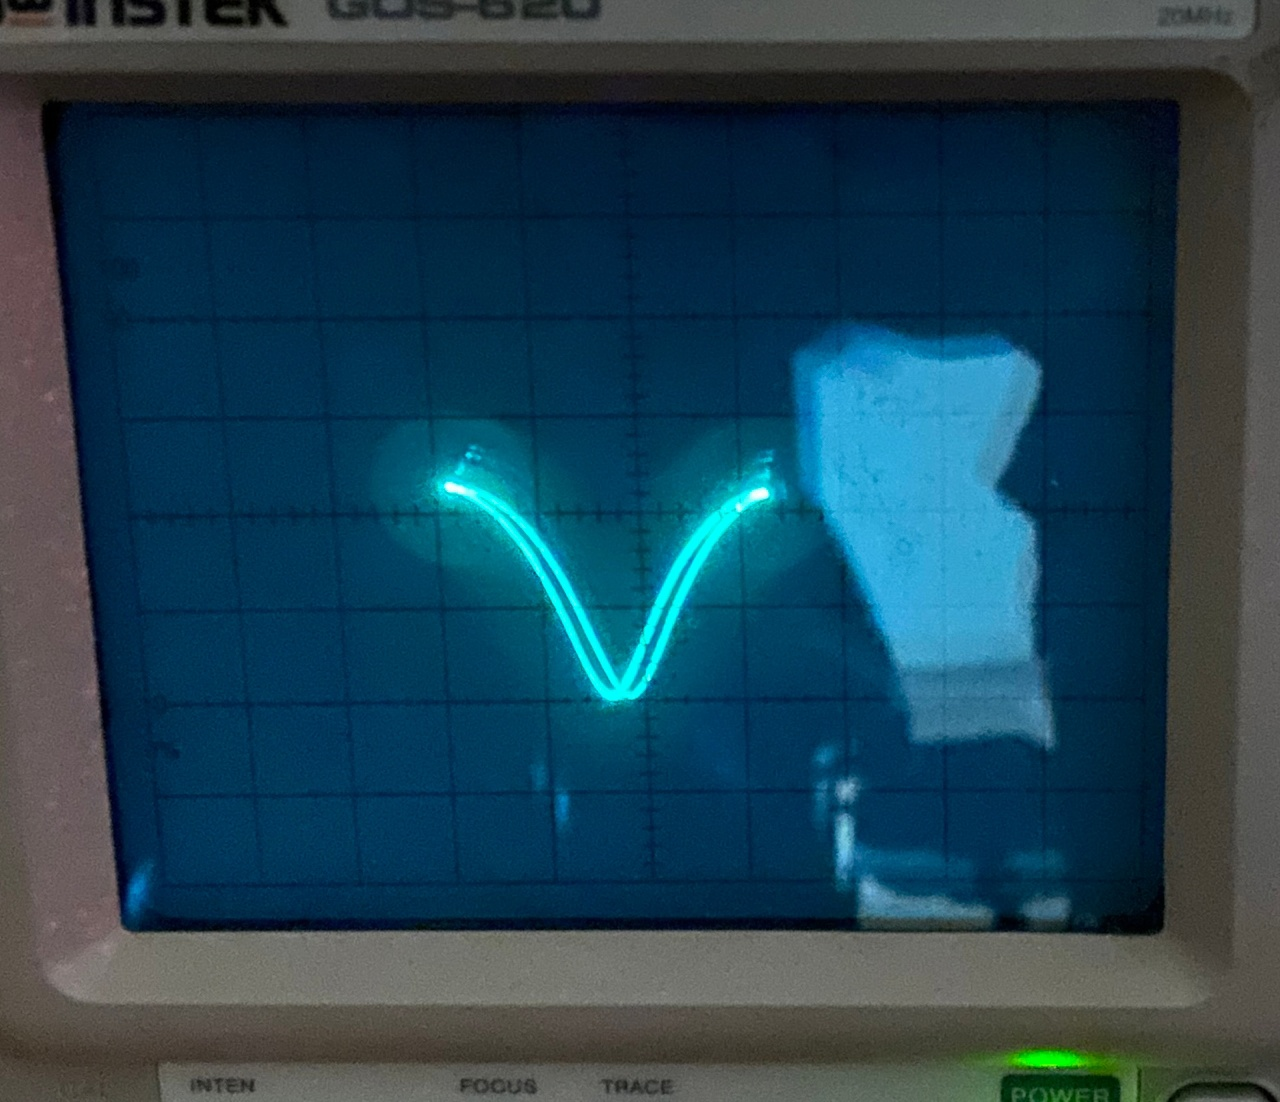
\includegraphics[width=0.8\textwidth]{p1}
    \caption{Перпендикулярная поляризация, $\lambda/2$}
    \label{fig:p1}
\end{figure}

\begin{figure}[H]
    \centering
    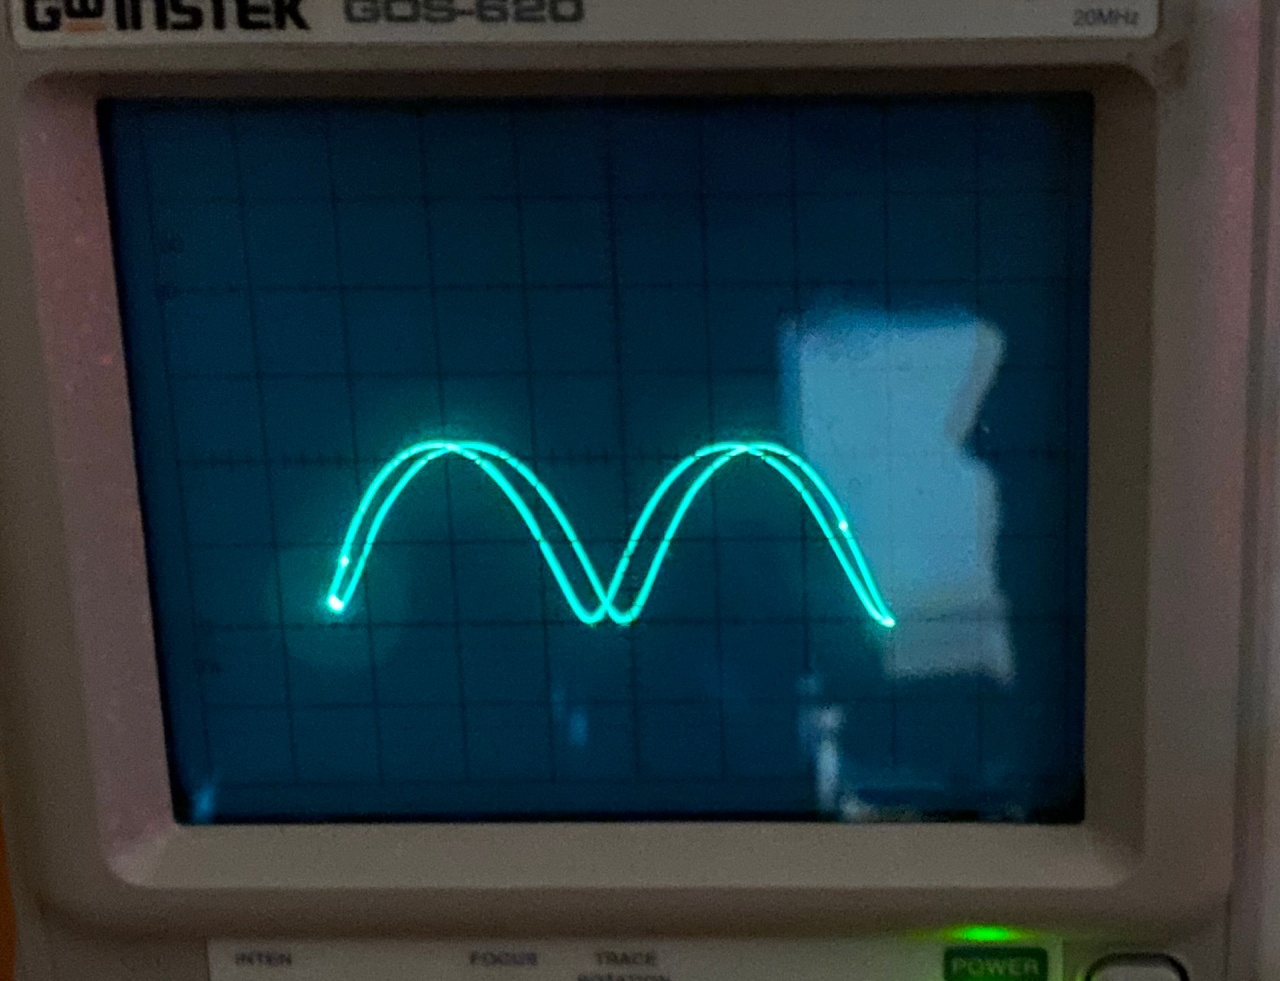
\includegraphics[width=0.8\textwidth]{p2}
    \caption{Перпендикулярная поляризация, $\lambda$}
    \label{fig:p2}
\end{figure}

\begin{figure}[H]
    \centering
    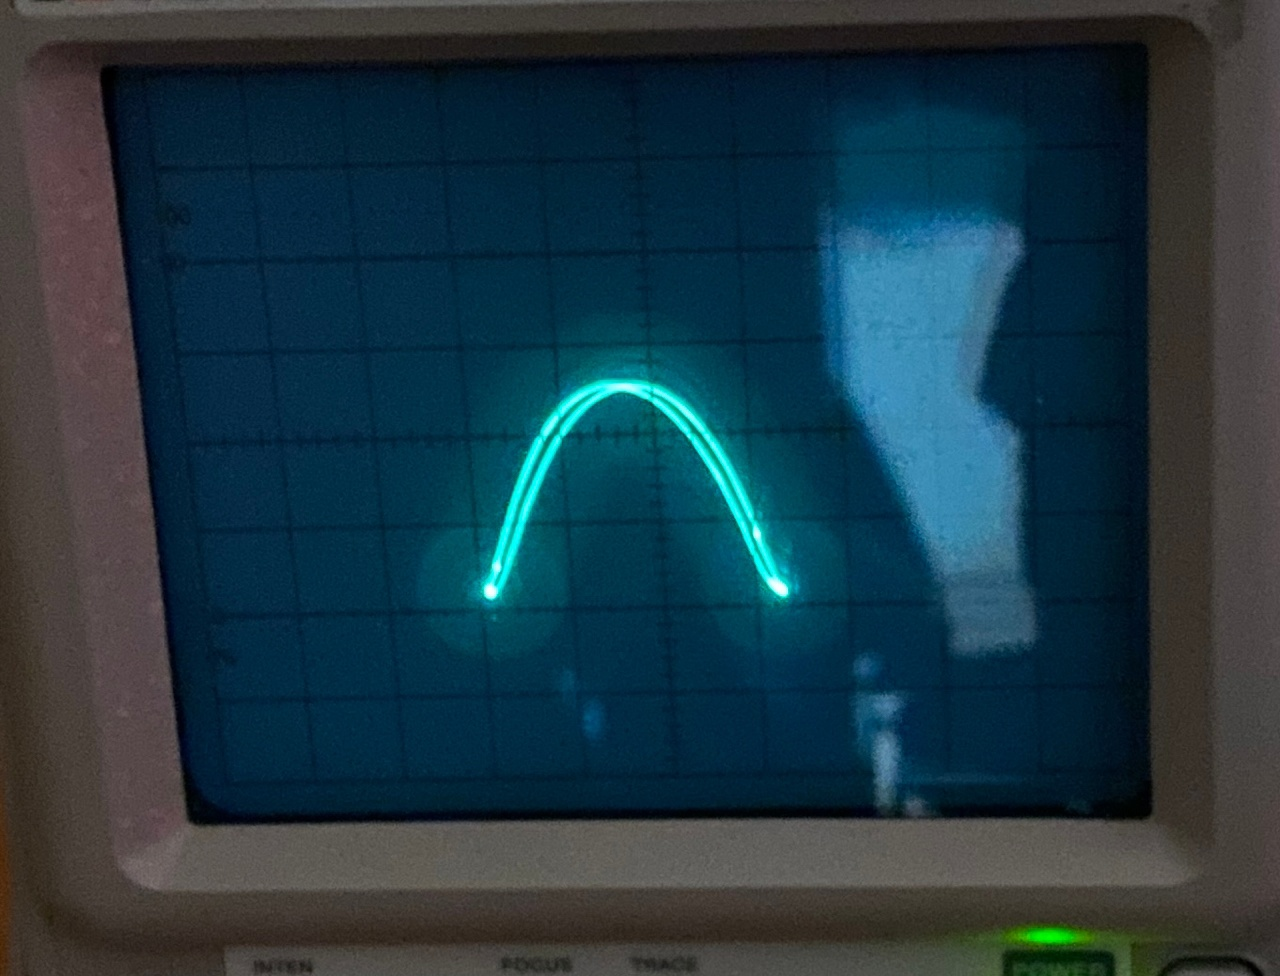
\includegraphics[width=0.8\textwidth]{i1}
    \caption{Параллельная поляризация, $\lambda/2$}
    \label{fig:i1}
\end{figure}

\begin{figure}[H]
    \centering
    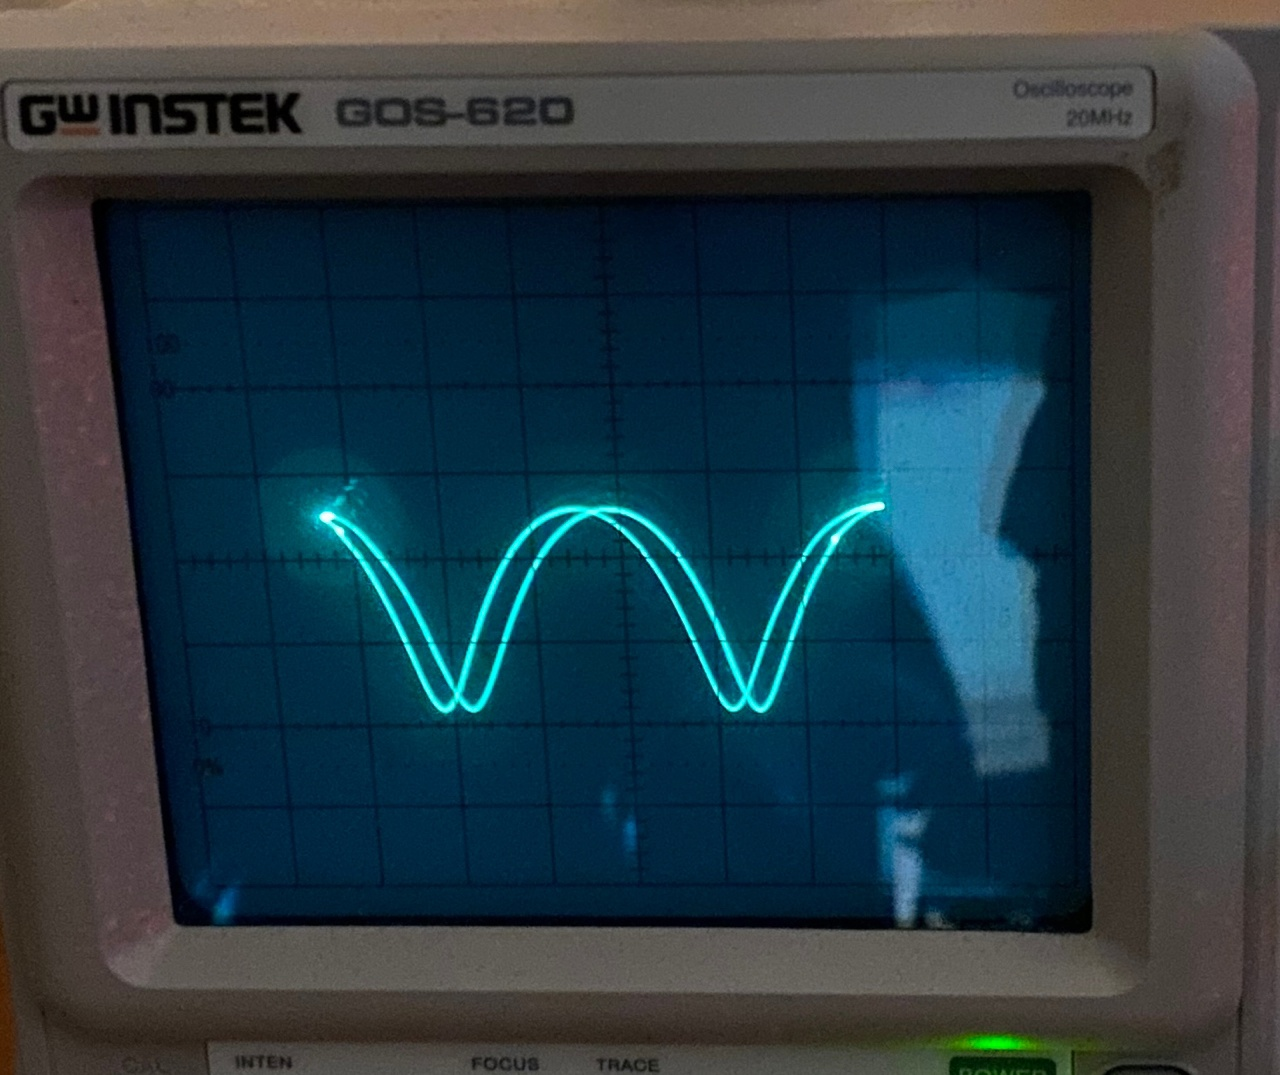
\includegraphics[width=0.8\textwidth]{i2}
    \caption{Параллельная поляризация, $\lambda$}
    \label{fig:i2}
\end{figure}

\section{Выводы}
В данной работе мы узнали что такое эффект Поккельса, получили интерференционную картину рассеянного света, прошедшего через кристалл $LiNbO_3$.
Было найдено значение для двулучепреломления $n_0 - n_e = 0,09 \pm 0,01$. Табличное значение составляет порядка $0,09$. 

Также были найдены полуволновые напряжения: $U_{\lambda/2} = 510 \pm 15$ В для постоянного тока и $U_{\lambda/2} = 420 \pm 15$ В для переменного тока. К тому же, мы убедились что при четвертьволновом напряжении имеет место круговая поляризация.

\end{document}